\documentclass[11pt]{paper}
\usepackage{fullpage}
\usepackage{graphicx}
\usepackage{palatino}
\usepackage{fancyhdr}
\usepackage{draftwatermark}
\usepackage{enumitem}
\usepackage{hyperref}
\setlist{nolistsep}

\renewcommand{\headheight}{0.4in}
\setlength{\headsep}{0.1in}

\setlength{\headwidth}{\textwidth}
\fancyhead[R]{\footnotesize m-labs.hk}
\fancyhead[L]{
   
\includegraphics[height=0.17in]{m_labs_logo.pdf}
}
\chead{}
\rfoot{}
\cfoot{\thepage}
\lfoot{}\pagestyle{fancy}

\begin{document}

\title{The Sinara device family}
\subtitle{high quality hardware for ARTIQ}
\author{S\'ebastien Bourdeauducq, Robert J\"ordens (M-Labs)}

\maketitle

\section{Background and objectives}
Control electronics used in many trapped-ion and other quantum physics experiments suffers from a number of problems. In general, an ad-hoc solution is hastily put together in-house without enough consideration about good design, reproducibility, testing and documentation. This makes those systems unreliable, fragile, and difficult to use and maintain. It also duplicates work in different laboratories. In addition, the performance and features of the existing systems (e.g.\ regarding pulse shaping abilities) is becoming insufficient for some experiments.

To alleviate those problems, M-Labs wish to propose high-quality and turnkey control hardware, which should be in particular:
\begin{itemize}
\item reproducible and open
\item flexible and modular
\item well tested
\item well supported by the ARTIQ control software
\end{itemize}

This document describes the desired components and features of this system.

We thank Joe Britton (ARL), Grzegorz Kasprowicz (Creotech/Warsaw University of Technology), David Leibrandt (NIST), and Daniel Slichter (NIST) for their valuable input.

\section{System overview}

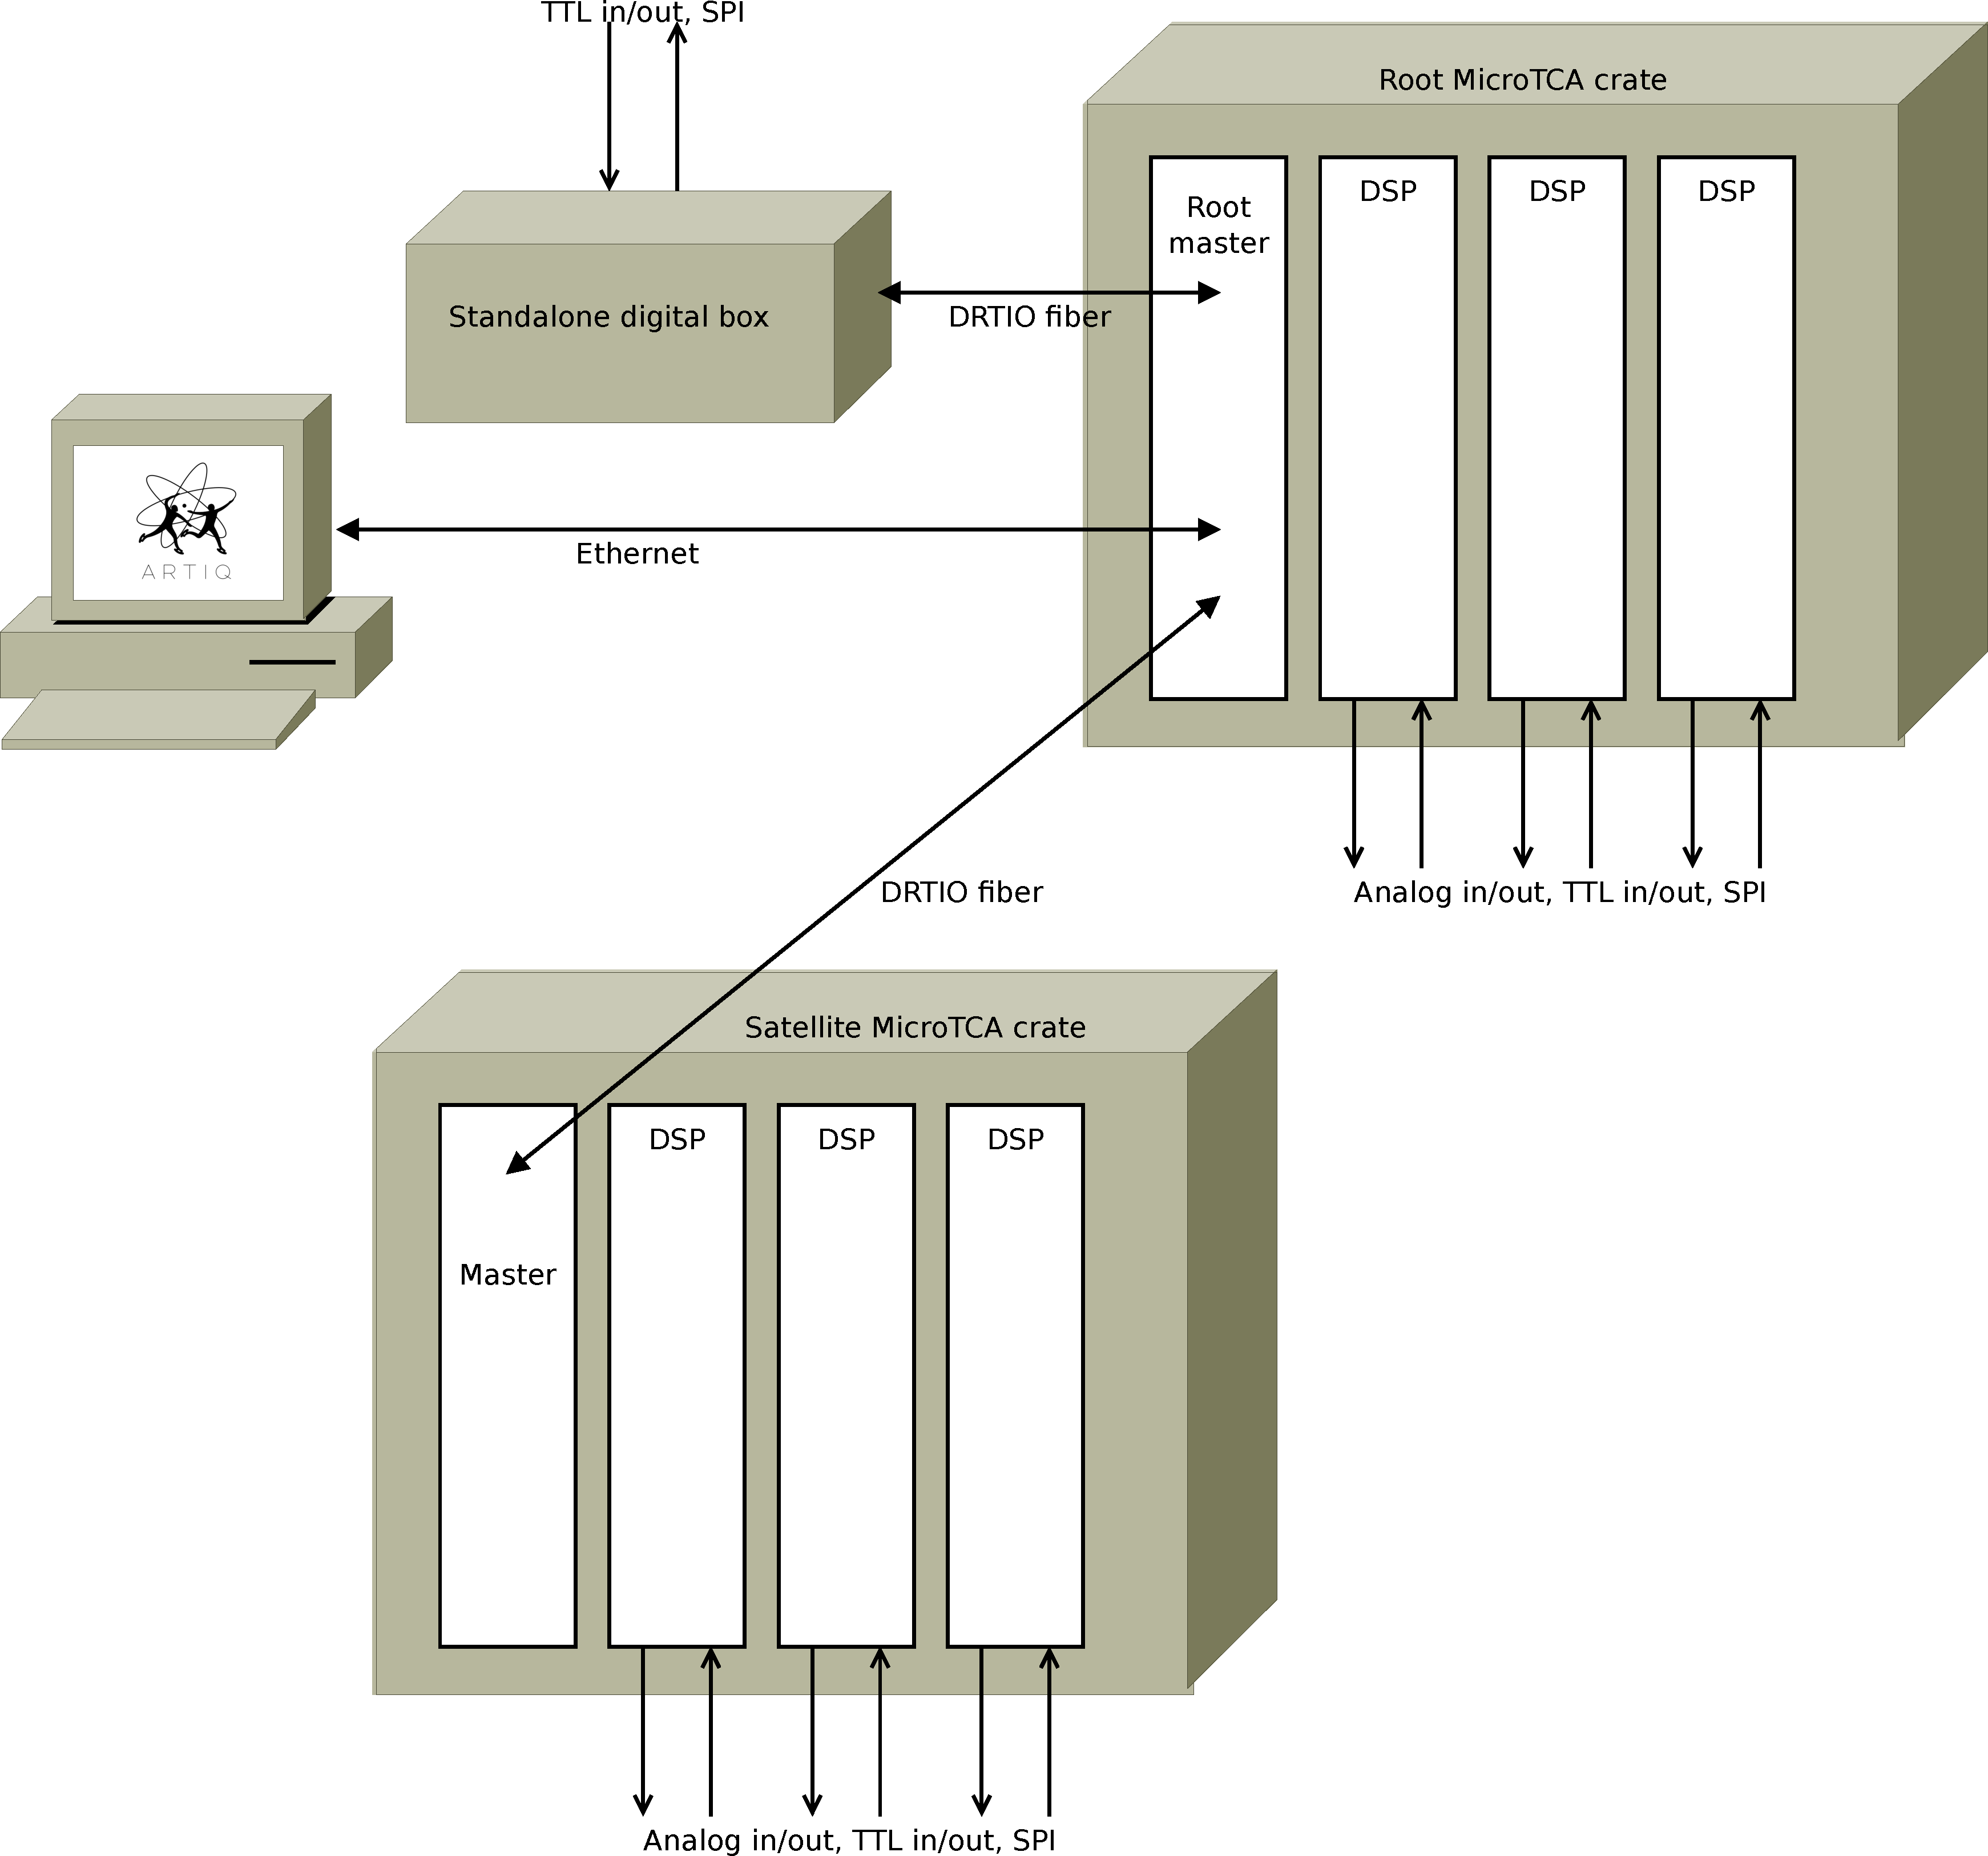
\includegraphics[width=\textwidth]{overview.pdf}

\section{MicroTCA crates}
The crates are compatible with the MicroTCA standard, and contain a power supply, cooling fans, a backplane (star topology), AMCs and MCH. In order to save space, and to keep all connectors on the same side, RTMs (MicroTCA.4) are not used and the crate should be chosen accordingly.

MicroTCA specifies a complicated ``IPMI'' management system. For compatibility reasons with other MicroTCA systems, the necessary hardware (a microcontroller circuit) should be present on the AMCs, but IPMI should otherwise be ignored as much as possible e.g.\ by keeping the power supplies on at all times.

To upgrade the gateware/runtime, firmware binaries are sent over the fiber or Ethernet for the FPGAs to write into their flash and reboot themselves, which is relatively simple and does not require additional hardware.

\section{Metlino boards}
A Metlino board is a double-width MicroTCA Carrier Hub (MCH) that:
\begin{itemize}
\item distributes DRTIO commands to the other cards in the crate over the MicroTCA backplane (star topology)
\item distributes DRTIO commands to other crates
\item receives commands from another Metlino board or the control PC
\end{itemize}

It has TBD SFPs on its front panel that are used for connecting to other devices (another Metlino board, TTL box, ...) over raw fiber optics, or to the control PC over Ethernet. The same fiber optic links may also be used for time transfer.

Metlino cards also have a digital I/O connector (VHDCI) on their front panel, that can be used to implement TTLs with little additional hardware.

A special Metlino board is the root master, which has the same role as the current core device in ARTIQ. It uses the same hardware as other master boards, but one of its SFPs is populated with a Ethernet PHY that is used to communicate with the control PC.

Metlino boards includes clock recovery and cleanup circuitry, and can be used to clock the other boards in the crate. A Metlino board also includes a SMA clock input connector on its front panel, in case the clock recovered from SFP is not of sufficient quality for the application, and for clocking the root master.

The FPGA used in Metlino boards is Kintex Ultrascale.

\section{Sayma boards}
The Sayma boards are double-width AMC cards that contain a FPGA, fast SDRAM (DDR4), and which are typically used to generate and process RF signals via high-speed DACs and ADCs.

The ADCs and DACs are mounted on external FMC cards called ``RF daughter cards''. The Sayma cards have two identical FMC slots, one may be used for transmitting signals (DACs) and one for receiving (ADCs).

The FMC connectors use the LPC pin assignments, plus 8 transceivers using the HPC pin assignments. Some HPC ground pins are repurposed to provide +5V, -5V, +15V and -15V to the FMC mezzanine cards. The use of ground pins (and current limits on the power supplies) prevents damage when incorrect FMC mezzanines are plugged. The Sayma cards also have jumpers that disable those power supplies so that regular LPC + HPC transceivers FMC cards can be plugged.

Sayma boards receive high level DRTIO commands from the backplane, and synthesize, buffer or process waveforms using their FPGA and SDRAM.

The SDRAM bandwidth must be sufficient to supply TBD spline knots per second to the waveform generator, corresponding to TBD Gbps.

The FPGA used in Sayma boards is Kintex Ultrascale XCKU040.

\section{RF daughter cards}
\subsection{Commonalities}
RF daughter cards are FMC cards that are mounted on Sayma carriers.

Output cards contain one JESD204 multi-channel high-speed DAC (AD9154, 4 channels in total).

Input cards contain one JESD204 multi-channel ADC (AD9656, 4 channels in total).

The synchronization signals of the DACs and ADCs must be accessible to the FPGA to support synchronization across multiple cards.

All output cards can be clocked from the FMC connector (which the DSP card can connect to a backplane clock, potentially through a PLL that upconverts it from 10-100MHz, TBD), and from a dedicated SMA connector on their front panel (selectable by jumper, solder, or digitally controlled switch). High-quality clock distribution systems using semi-rigid coaxial cables can be used for particularly sensitive applications. The clock connector can also be used to experiment with different clocking systems. The output cards thus have 5 SMA connectors on the front panel, which is the maximum number that fit in that limited space.

Input cards may omit the external clock connector, as the ADCs are slower and the applications are less sensitive to clock noise when acquiring signals.

Input and output cards come in simple versions that contain only the basic circuitry plus an area that can receive a user-designed castellated module. Footprints for the castellated modules may be similar to those used by Marki Microwave.

TBD: we may want to have 8 DAC channels per Sayma card instead, have the DAC/ADC chips on the Sayma, and use something else than FMC.

\subsection{Karabash simple output card}
The four DAC channels are connected to pads that can receive a castellated prototyping module. The output card also has four SMA connectors on its front panel (in addition to the clock connector), with traces to the castellated module.

As part of this project, we shall provide a pass-through castellated module that connects the DACs directly to the SMA connectors.

\subsection{Ulvidy low frequency output card}
Signal bandwidth of a few MHz, swinging between +/- 10 V or so, suitable for ion trap transport waveforms or various DC or quasi-DC bias signals in general applications. This would involve op amps/instrumentation amps running off +/- 15V supplies in a similar configuration to the current PDQ output stages. Footprints for discrete component filters both before and after the amplifiers should be included.

\subsection{Argayash RF output card}
For synthesis of tones from a few MHz out to about 3.3 GHz, suitable for AOM drive, or Be\textsuperscript{+}, Mg\textsuperscript{+}, Ca\textsuperscript{+} and NV center microwave transitions. This would involve a set of filters (common footprint, stuff boards with different cutoff parts to define band of interest -- these can be left open for users, or we can choose one or two basic frequency sets and they can run their own custom assembly order from the fab/layout docs if they want something different, TBD) followed by an RF amplifier stage (ERA-4SM is a good broadband low-phase-noise selection), a digital step attenuator, and a fast high-isolation RF switch.

\subsection{Tatysh upconverting output card}
For synthesis of tones beyond about 3.3 GHz, suitable for Yb\textsuperscript{+} or superconducting qubit microwave transitions. The board would have an input connector for an externally generated microwave carrier, split and sent to the LO ports of a set of mixers/modulators. We should decide (TBD) if these needs to be IQ mixers or if regular mixers are sufficient. There will be filters (again, common footprint for a choice of frequencies) between the DAC outputs and mixer IF ports. Each mixer RF port will be followed by an amplifier, a digital step attenuator, and a fast high-isolation RF switch.

\subsection{Allaki simple input card}
The four ADC input channels go through a signal conditioner (amplifiers/attenuators) configurable by the FPGA (variable gain) before they reach a castellated module. The card has four SMA connectors on the front panel that are connected to the castellated module.

As part of this project, we shall provide a pass-through castellated module that connects the signal conditioner directly to the SMA connectors.

\subsection{Sayma gateware/runtime specification}
%% \section*{ARTIQ-SAYMA\footnote{Smart ArbitrarY waveform ModulAtor}}

\paragraph{Overview}

Specification and design concept for a high data rate, multi-tone, interpolating, scalable, smart, high-speed arbitrary waveform generator.

\paragraph{Spline parametrization}

\emph{This is inherited from the \href{http://pdq2.readthedocs.io/en/latest/}{pdq2 documentation}}

The method of compression is a polynomial basis spline (B-spline).
The data consists of a sequence of knots. Each knot is described by
a duration $\Delta t$ and spline coefficients $u_{n}$ up to order
$k$. If the knot is evaluated starting at time $t_{0}$, the output
$u(t)$ for $t\in[t_{0},t_{0}+\Delta t]$ is
$$
u(t)=\sum_{n=0}^{k}\frac{u_{n}}{n!}(t-t_{0})^{n}=u_{0}+u_{1}(t-t_{0})+\frac{u_{2}}{2}(t-t_{0})^{2}+...
$$
A sequence of such knots describes a spline waveform. From one discrete
time $i$ to the next $i+1$ each accumulator $v_{n,i}$ is incremented
by the value of the next higher order accumulator:
$$
v_{n,i+1}=v_{n,i}+v_{n+1,i}
$$
For a cubic spline the mapping between accumulators' initial values
$v_{n,0}$ and the polynomial derivatives or spline coefficients $u_{n}$
can be done off-line and must take into consideration the finite time
step size $\tau$. The data for each knot is described by the integer
duration $T=\Delta t/\tau$ and the initial values $v_{n,0}$. This
representation allows both transient large-bandwidth waveforms
and slow but smooth large duty cycle waveforms to be described very efficiently.

\paragraph{Waveform parametrization}

The gateware will support at least 8 independent channels.

Each channel emits waveforms of the general parametrization:
$$
	z=\left( a_1e^{i(f_1 t+p_1)} + a_2e^{i(f_2 t+p_2)}\right)e^{i(f_0t+p_0)}
$$
$$
	o=u+b_0\mathrm{Re}(z)+b_1\mathrm{Im}(z^\prime)
$$

\begin{itemize}
	\item $o$ is the (real valued) output of a channel
	\item $z$ is the complex-valued output of the ``generator'' associated with each channel
	\item $z^\prime$ is the complex-valued output from the generator of each channel's ``buddy'' channel.
		Two adjaccent channels form a buddy pair.
		This enables seamless usage of the complex data path features in DACs, complex (IQ) analog modulation, and yields ``four-tone'' support on IQ channels for free.
	\item $u$ and $a$ are 16-bit cubic (third order) spline interpolators
	\item $p$ are 16-bit constant (zeroth order) spline interpolators
	\item $f$ are 48-bit linear (first order) interpolators
	\item $b$ are switches ($1$ or $0$)
\end{itemize}

\paragraph{Datapath details}

\begin{itemize}
	\item $f_\mathrm{DATA}\geq1\,\mathrm{GHz}$. Exact clock speed is TBD and depends on simultaneously meeting hardware constraints and an integer relationship with the RTIO clock and physics/noise requirements.
	\item Oscillator $f_0,p_0$ is sampled at $f_{DATA}$
	\item Interpolators are updated and interpolate at $f_\mathrm{DATA}/k$ with $k$ typically 4 or 8 and $f_\mathrm{DATA}/k \geq 125\,\mathrm{MHz}$
	\item Oscillators $f_{1,2},p_{1,2}$ are sampled at $f_{DATA}/k$
	\item All amplitude summing junctions shall implement saturating summation to prevent wrap-around.
	\item All amplitude summing junctions shall implement configurable and guaranteed gateware low-high limiters.
	\item All amplitude summing junctions shall register saturation events.
	\item To up-sample the data from the $f_1$,$f_2$ oscillators by $k$ before passing it into the $f_0$ oscillator, a CIC filter of order TBD shall be implemented for anti-aliasing. CIC filters are linear phase.
	\item To implement further anti-aliasing, a symmetric (thus linear phase) FIR filter with TBD taps (FPGA DSP resource limits) shall be implemented after the CIC filter.
	\item All spline interpolators and the total channel output shall be monitored by the ARTIQ channel monitoring infrastructure.
	\item All spline interpolators shall support ARTIQ injection/override.
\end{itemize}

\paragraph{Clocking and synchronization}

\begin{itemize}
	\item Timestamps for spline knot scheduling are at least 62 bit wide.
	\item Spline knots have 16-bit dynamic range in time.
	\item In order to support slower sweeps with sparser spline knots, the dynamic range of the spline coefficients can be extended using time stretcher.
		It decelerates the spline evolution/interpolation rate by a factor of $2^E$.
	\item Waveform output shall be with deterministic latency with respect to the RTIO clock:
		\begin{itemize}
			\item across channels on the same card (to within DAC
				chip specification)
			\item across cards in the same rack (to within DAC chip
				and intra-rack DRTIO clock sycnchronization)
			\item across racks controlled by the same core device
				(to within DAC chip and DRTIO clock synchronization)
		\end{itemize}
	\item Each card can be clocked by an internal DAC clock derived from the RTIO clock or by an external DAC clock.
	\item When an external DAC clock is used, the waveform synchronization is ensured to within one DAC clock cycle (or the limit of the DAC chip whichever is higher) but below that depends on the phase of the external DAC clock.
	\item All spline knot interpolators can be updated independently (and also simultaneously) of each other.
	\item All spline interpolator latencies from the internal ``RTIO clock reference plane'' to the DAC output are matched and deterministic.
		Channel and board latencies are matched and deterministic (see above).
	\item Minimum spline knot duration is $k/f_\mathrm{DATA}$. 
\end{itemize}

\paragraph{Phase update modes}

The phase accumulator of the DDS cores can be updated in multiple different modes during a phase and/or frequency update.

\begin{itemize}
	\item relative phase update: $q^\prime(t) = q(t^\prime) + (p^\prime - p) + (t - t^\prime) f^\prime$
	\item absolute phase update: $q^\prime(t) = p^\prime + (t - t^\prime) f^\prime$
	\item phase coherent update: $q^\prime(t) = p^\prime + (t - T) f^\prime$, where
	\item $q$/$q^\prime$: old/new phase accumulator
	\item $p$/$p^\prime$: old/new phase offset
	\item $f^\prime$: new frequency
	\item $t^\prime$: timestamp of setting new $p$,$f$
	\item $T$: ``origin'' timestamp: beginning of experiment, boot of device, or arbitrary
	\item $t$: running time
\end{itemize}

Relative phase updates are called ``continuous phase mode'' and coherent updates are called ``tracking phase mode'' by some.
Phase coherent updates can be mapped (in software/runtime) to absolute phase updates by transforming $p^\prime \longrightarrow p^\prime + (t^\prime - T) f^\prime$.
Since phase coherent updates require large multiplications is is questionable whether they can and should be implemented in gateware.

It is questionable whether phase coherent updates should or even can be supported for sweeping $p$/$f$. They can be supported for the modulation inputs (see below).

\paragraph{Modulation by RTIO}

To each spline interpolator (any of the nine $f,p,a,u$ in the waveform
parametrization) a modulation (summarized as $e_\mathrm{RTIO}$) by a separate RTIO channel can be applied.


\begin{itemize}
	\item The modulation is an additive offset for frequency and phase ($f,p$) and a multiplicative offset for amplitudes ($u,a$).
	\item The modulation is times like any other (non-interpolating) RTIO event, i.e. $\leq 8$\,ns time resolution and has the same value resolution as the spline interpolator it modulates.
	\item Default values are 0 for frequency and phase modulation ($f,p$) and 1 for amplitude modulation ($u,a$).
	\item Modulation is normalized to full scale.
\end{itemize}

\paragraph{Modulation by local DSP}
In addition to RTIO modulation $e_\mathrm{RTIO}$ there is ``local DSP'' modulation
input to each spline interpolator.

\begin{itemize}
	\item Same specifications and semantics as the RTIO modulation.
\end{itemize}

\paragraph{Local DSP}
A fully reconfigurable local DSP fabric with multiple IIR filters shall be
included. The DSP switchyard supports servoing applications of various types.
\begin{itemize}
	\item See \href{https://github.com/jordens/redpid}{redpid} for a rough
		feature set.
\end{itemize}

\paragraph{Runtime and kernel interface}
\begin{itemize}
	\item Spline knot sequences can be generated off-line and embedded in ARTIQ experiments.
	\item Spline knot sequences can be generated at compile time.
	\item Spline knot sequences can be embedded into ARTIQ experiments and emitted to from the core device to the DRTIO channels during the experiments.
	\item Spline knot sequences can be computed dynamically on core device.
	\item Instead of emitting them directly to the DRTIO channel, spline knot sequences can be emitted into a named DMA context which stores the RTIO events in memory (either on the core device or right at the DRTIO channel in the card's DRAM) for later recall.
	\item Stored, named DMA segments can be replayed by name.
	\item Given enough slack to transmit DRTIO events and fill the channel FIFOs (from core device or from any DMA source), all boards, all channels, all splines can burst $\geq128$ knots each at $\geq125$\,MHz (BRAM FIFO limited). This is independent of whether the events are computed dynamically, off-line, embedded, reside in core device DRAM or remote DRAM.
	\item When sourcing waveforms from core device memory, the sustained aggregated spline knot rate across all interpolators is $\geq2$\,MHz.
	\item Sourcing from remote DRTIO DMA the spline knot rate per board (aggregated over all channels and all interpolators on that board) is TBD MHz sustained for TBD knots (DRAM limited).
	\item Supports setting $e_\mathrm{DRTIO}$ using standard DRTIO events.
	\item Supports configuring the DAC through RTIO-SPI
	\item Utility functions shall be made available to users for processing spline waveforms (scaling in value and time, resampling).
	\item Given a periodically sampled waveform (vector of values) routines shall
	\begin{itemize}
		\item generate a spline waveform with a fixed knot duration 
		\item generate a spline waveform with specified knot count and variable knot duration 
		\item generate a spline waveform with minimal knot count and specified RMS error
	\end{itemize}
	\item given user-supplied spline waveform routines shall
	\begin{itemize}
		\item generate a periodically sampled waveform (vector of values) with user specified resolution
		\item determine validity (in-range)
	\end{itemize}

\end{itemize}

\paragraph{Test Cases}

ARTIQ Python programs demonstrating the following will be provided.

\begin{enumerate}
	\item Simultaneous generation of two-tone waveforms on 8 DAC channels where $f_{1}=f_{0}+\Delta$ and $f_{2}=f_{0}-\Delta$ where $f_{0}=200$~MHz and $\Delta=[0,50]$~MHz.
	\item Playing a spline knot sequence demonstrating each spline interpolator in
		turn.
	\item Replaying a 128 knot two-tone amplitude sequence from remote DMA.
	\item Phase/frequency/amplitude shifting that sequence using $e_\mathrm{DRTIO}$.
	\item Demonstrate relative and absolute phase mode.
	\item Demonstrate deterministic channel alignment to one DAC clock cycle.
	\item Demonstrate external and internal clocking.
\end{enumerate}

\section{Kasli boxes}
The Kasli boxes receive DRTIO commands (and optionally time) over a SFP and fiber connected to a master card, and generate and receive TTL pulses and digitally control devices such as SPI integrated circuits. They have TBD SMA connectors and TBD RJ45 connectors that can be connected to e.g.\ SPI devices. They contain their own power supply.

The Kasli boxes also have a dedicated clock input SMA connector, that can override the clock recovered from the SFP.

For convenience, the boxes also contain one AD5370 SPI DAC with its 40 channels connected to a D-sub connector (e.g.\ DD-50).

The FPGA used in Kasli boxes is XC6SLX45T or XC7A100T.

\section{Sayma/Metlino FPGA choice}

There are several constraints and interfaces that need to be satisfied by the FPGAs used for Metlino and Sayma.

\paragraph{Manufacturer and Experience} M-Labs has accumulated significant experience with Xilinx programmable logic devices over the last decades.
They generally are among the most advanced devices available closely tracking the latest technology node in semiconductor development.

\paragraph{Compatibility} ARTIQ has focused on Xilinx Spartan 6 and Kintex 7 families so far.
A move to a new family would require targeting new logic interfaces like transcievers or IOSERDES and new development boards.

\paragraph{Consolidation} It is advantageous to reuse chips from the same device family or even the same chip in as many components of the ARTIQ hardware ecosystem as possible.
Same dies in the different packages require no bitstream changes and no additional bitstream build/testing and maintenance overhead.
Different speed grades of the same die and package do not require board
changes.
Using footprints where different sizes are available in compatible pin-outs would enable swapping chips without altering boards in response to growing needs for logic and other resources.

\subsection{Resources available}

The following table collates the most relevant resources of previous, present, and potential future FPGA devices that could be targeted in Sayma and Metlino.
The amount of standard IOs are not expected to be a limiting resource.
Nor do we anticipate the need for other hard-silicon resources like PCIe, memory controller, or CPU blocks.

\noindent
\begin{tabular}{l|llll}
   device   & LUT  & BRAM  & DSP  & transciever   \\\hline
   xc6s45t  & 27k  & 2\,Mb   & 58   & 4 GTP (3.2\,GHz)   \\
   xc7a100t-2 & 63k  & 4.9\,Mb & 240  & 8 GTP (6.6\,GHz)  \\
   xc7z010  & 18k  & 0.2\,Mb & 80   & -              \\
   xc7k325t-2 & 200k & 16\,Mb  & 0.8k & 16 GTX (10.3\,GHz) \\
   xc7k410t & 250k & 29\,Mb  & 1.5k & 16 GTX         \\
   xcku040  & 242k & 21\,Mb  & 1.9k & 20 GTH (12.5\,GHz) \\
   xcku060  & 330k & 38\,Mb  & 2.8k & 32 GTH         \\
   xcku095  & 550k & 60\,Mb  & 0.8k & 32 GTH, 32 GTY \\
\end{tabular}

\subsection{Resource requirements}

\subsubsection{Front panel real estate}

\paragraph{Sayma} A mid-size AMC is the standard board size for MicroTCA crates. Full-size AMC crates do not appear to be commonly available.
RF connectors at the front panel need a sufficient spacing to be accessible for mounting.
The 4 HP spacing of mid-size AMC is barely sufficient spacing to allow for mounting SMA connectors with proper application of torque and without damaging the equipment.
Other connectors that do not require screws would be easier to mount.

Assuming the standard front panel layout of mounting mechanisms and LEDs, there seems to be just about enough space for eight SMA connectors on the front panel of a double-width AMC.
Potentially nine, if a separate clock input is required.

The usability would be severely limited if significantly more connectors are added to the Sayma front panel.

\paragraph{Metlino} There is space for four SFP cages, LEDs, and clock inputs
on a single width MCH.

\subsubsection{Sayma SAWG data rate constraints}

The fast smart arbitrary waveform channels require a significant amount of logic resources but also necessitate fulfilling several interacting constraints on operating frequencies and clock ratios.

For the DAC channel data rate $f_\mathrm{DATA}$ on the JESD204B link, the following rules need to be observed.

\begin{itemize}
   \item $t_\mathrm{DATA} = t_\mathrm{RTIO\_FINE}$. DAC samples need to mesh with RTIO timestamps (e.g. RF switches on TTLs and SYS\_REF tagging), otherwise DAC timing is not sample-accurate and samples will beat around RTIO timestamps.
      The RTIO timestamp granularity is a global design variable of an ARTIQ DRTIO fabric instance.
      The granularity does not need to be 1\,ns and can easily be altered globally, but it needs to be the same across the entire DRTIO fabric.
      If e.\,g. the core device has a coarse clock of 125\,MHz and the high resolution TTL provide three more bits of resolution, then the fine timestamp granularity needs to be 1\,ns (or an integer submultiple) everywhere.
    \item $t_\mathrm{SLOWDDS}/k = t_\mathrm{FASTDDS} = t_\mathrm{DATA}$ with $k$ a power of two. The accumulator phasing and datapath parallelization methods that allow generating multiple samples in a single clock cycle only work for powers of two.
    \item $t_\mathrm{SLOWDDS}$ can potentially be as low as 4\,ns on Kintex 7 with speed grade 2 or better, certainly as low as 5\,ns. The possibility of 4\,ns fabric timing would need to be explored and verified.
    \item $t_\mathrm{SLOWDDS} = m t_\mathrm{RTIO\_FINE}$: The spline interpolators, RTIO updates, and the slow DDS should mesh with the fine timestamp (e.g. RF switches on TTLs).
    \item $t_\mathrm{SLOWDDS} = p t_\mathrm{RTIO}$: The spline interpolators, RTIO updates, and the slow DDS should mesh with the coarse timestamp (e.g. relative to RF switches on coarse TTLs). $p$ is a power of two in the current ARTIQ architecture.
    \item $f_\mathrm{DATA} \leq 1.09\,\mathrm{GHz}$ or even $ \leq
       1.03\,\mathrm{GHz}$ for typical DAC and FPGA transciever line rate.
\end{itemize}

The DAC sample rate $f_\mathrm{DAC}$ after interpolation and up-sampling from $f_\mathrm{DATA}$ needs to satisfy:

\begin{itemize}
   \item $f_\mathrm{DATA} \leq 2.4\,\mathrm{GHz}$: Typical DAC sample rate
   \item $f_\mathrm{DAC} = q f_\mathrm{DATA}$ with $q \in \{1, 2, 4, 8\}$: Available interpolation options
\end{itemize}

\subsubsection{FPGA logic resources}

\paragraph{Transcievers}

\begin{itemize}
   \item Sayma DRTIO: one GTX/GTH upstream, rest downstream.
   \item Metlino DRTIO: 12 or 6 GTX/GTH downstream to supplie 12 or 6 AMC cards in a rack. One GTX/GTH upstream. At least one downstream: 14 or 8 transcievers total.
   \item Sayma DAC, currently AD9154: 8 JESD204B lanes, 8 GTX/GTH TX halves, 10 GHz line rate: speed grade -2 xc7k, any on xcku
   \item Sayma ADC: 4 GTX/GTH RX halves
\end{itemize}

\paragraph{Logic and RAM}

\begin{itemize}
   \item ARTIQ device CPU(s) and miscellaneous logic resources provide a good  estimate for the additional logic required to support DRTIO.
      The kc705-nist\_qc2 design occupies 23k LUT and 5\,Mb BRAM.
      The pipistrello-nist\_qc1 design uses 15k LUT and 1\,Mb BRAM (on a slightly different architecture).
    \item parallelized FIR: 4 channel, 4x parallelism, 30 taps: 240 DSP
    \item parallelized HBF + tricks: 4 channel, 4x parallelism, 30 taps: 120 DSP
    \item RTIO FIFOs: 4 channel, 128 knots per RTIO channel: 4Mb
   \item PID, extrapolating from redpid (xc7z010): 2 channel 125MHz ADC/DAC + misc DSP, full servo crossbar matrix: 13 kLUT, 50 DSP
\end{itemize}

Several design studies were performed for different configurations of the Sayma SAWG channels:

\begin{itemize}
    \item Sayma initial SAWG on kc705: 2 channel, 8x parallelism, 125MHz: 28k LUT
    \item Sayma advanced draft SAWG on kc705: 4 channel, 4x parallelism, 200MHz: 33k LUT
    \item Sayma advanced draft SAWG on kc705: 4 channel, 8x parallelism, 125MHz: 53k LUT
    \item Sayma advanced draft SAWG on kc705: 8 channel, 8x parallelism, 125MHz: 106k LUT
    \item Sayma advanced draft SAWG on kcu105: 4 channel 4x parallelism, 200MHz: 33k LUT
\end{itemize}

\subsection{Prototyping options}

For development and differential debugging with hardware prototypes it is highly desirable to have access to a development/evaluation board that uses similar components as Sayma and Metlino.
The following devices are the prominent choices:

\paragraph{KC705}

Containing a xc7k325t it is the primary ARTIQ prototyping platform.
Almost all of the relevant hardware is supported or will be in the near future.
In order to support the Metlino Ethernet uplink the following would need to be developed:

\begin{itemize}
   \item A transciever-based Ethernet PHY to support communication of the core
      device with the PC (SFP module).
\end{itemize}

This is of medium complexity and cost.

\paragraph{AFCK}

Similar to the KC705, the board support package (BSP) would \emph{additionally} require support for:

\begin{itemize}
   \item (minor) JTAG mux
   \item (minor) rack management/IPMI
\end{itemize}

Both appear to be of minor complexity and cost.

\paragraph{KCU105}

The KCU105 is built around a xcku040 Kintex Ultrascale.
Supporting the FPGA and the relevant components of the board would necessitate developing support for:

\begin{itemize}
    \item DDR4 memory and controller
    \item GTH transcievers for DRTIO
    \item Copper ethernet PHY (SGMII) or transciever based using GTH+SFP
    \item (minor) IOSERDES (for high-resolution TTL channels)
    \item (minor) multiple flash layout/JTAG
\end{itemize}

The first three items are of medium complexity and cost.

\subsection{Recommendation}

\paragraph{FPGA choice} Judging from the resource requirements and constraints listed above, the available FPGAs can be classified by their applicability to Metlino, Sayma, and Kasli as follows:

\noindent
\begin{tabular}{l|lllll}
   & xc6s45t & xc7a100t & xc7k325t & xcku040 \\\hline
   Sayma 4 ADC, 4 DAC & insufficient & insufficient & good & overkill \\
   Sayma 8 ADC, 8 DAC & insufficient & insufficient & insufficient & good \\
   Metlino 12 AMC & insufficient & insufficient & good & good \\
   Metlino 6 AMC & insufficient & insufficient & good & overkill \\
   Kasli & good & good & overkill & overkill\\
\end{tabular}

\paragraph{Data and sample rates} The following choices for data rates and
lanes appear to be interesting (BW: bandwidth; SSB: single sideband; DSB: dual
sideband):

\noindent
\begin{tabular}{llllllll}
   $f_\mathrm{DAC}$ & $f_\mathrm{DATA}$ & line rate
   & lanes & $f_1,f_2$ DSB BW & $f_0$ SSB BW & BW mix 2nd+3rd \\\hline
   2.4\,GHz & 600\,MHz & 6\,GHz & 8 & 150\,MHz & 0--300\,MHz & 300--900\,MHz \\
   2\,GHz & 1000\,MHz & 10\,GHz & 8 & 125\,MHz & 0--500\,MHz & 500--1500\,MHz \\
   1.6\,GHz & 800\,MHz & 8\,GHz & 8 & 200\,MHz & 0--400\,MHz & 400--1200\,MHz \\
   300\,MHz & 300\,MHz & 6\,GHz & 4 & 150\,MHz & 0--150\,MHz & 150--450\,MHz \\
\end{tabular}

For 4 JESD lanes, use DAC ``mix mode'' (switching up-conversion by $f_\mathrm{DAC}$) to
emphasize second Nyquist zone from $f_\mathrm{DAC}/2$ to $f_\mathrm{DAC}$. Zeros at 0\,Hz
and $2\times f_\mathrm{DAC}$.

\end{document}
